\newpage
%\pagestyle{empty}

\begin{minipage}[c]{.25\linewidth}
	
\includegraphics[width=4cm]{images/Logo-LEnsE.png}
\end{minipage} \hfill
\begin{minipage}[c]{.4\linewidth}

\begin{center}
\vspace{0.3cm}
{\Large \textsc{Interféromètre de ZYGO}}

\medskip

\textbf{\Large IHM - \textsc{Généralités}}

\end{center}
\end{minipage}\hfill

%%%%%%%%%%%%%%%%%%%%%%%%%%%%%%%%%%
\section{Structure de l'interface}

L'interface de contrôle de l'interféromètre de Zygo se présente ainsi :

\begin{center}
	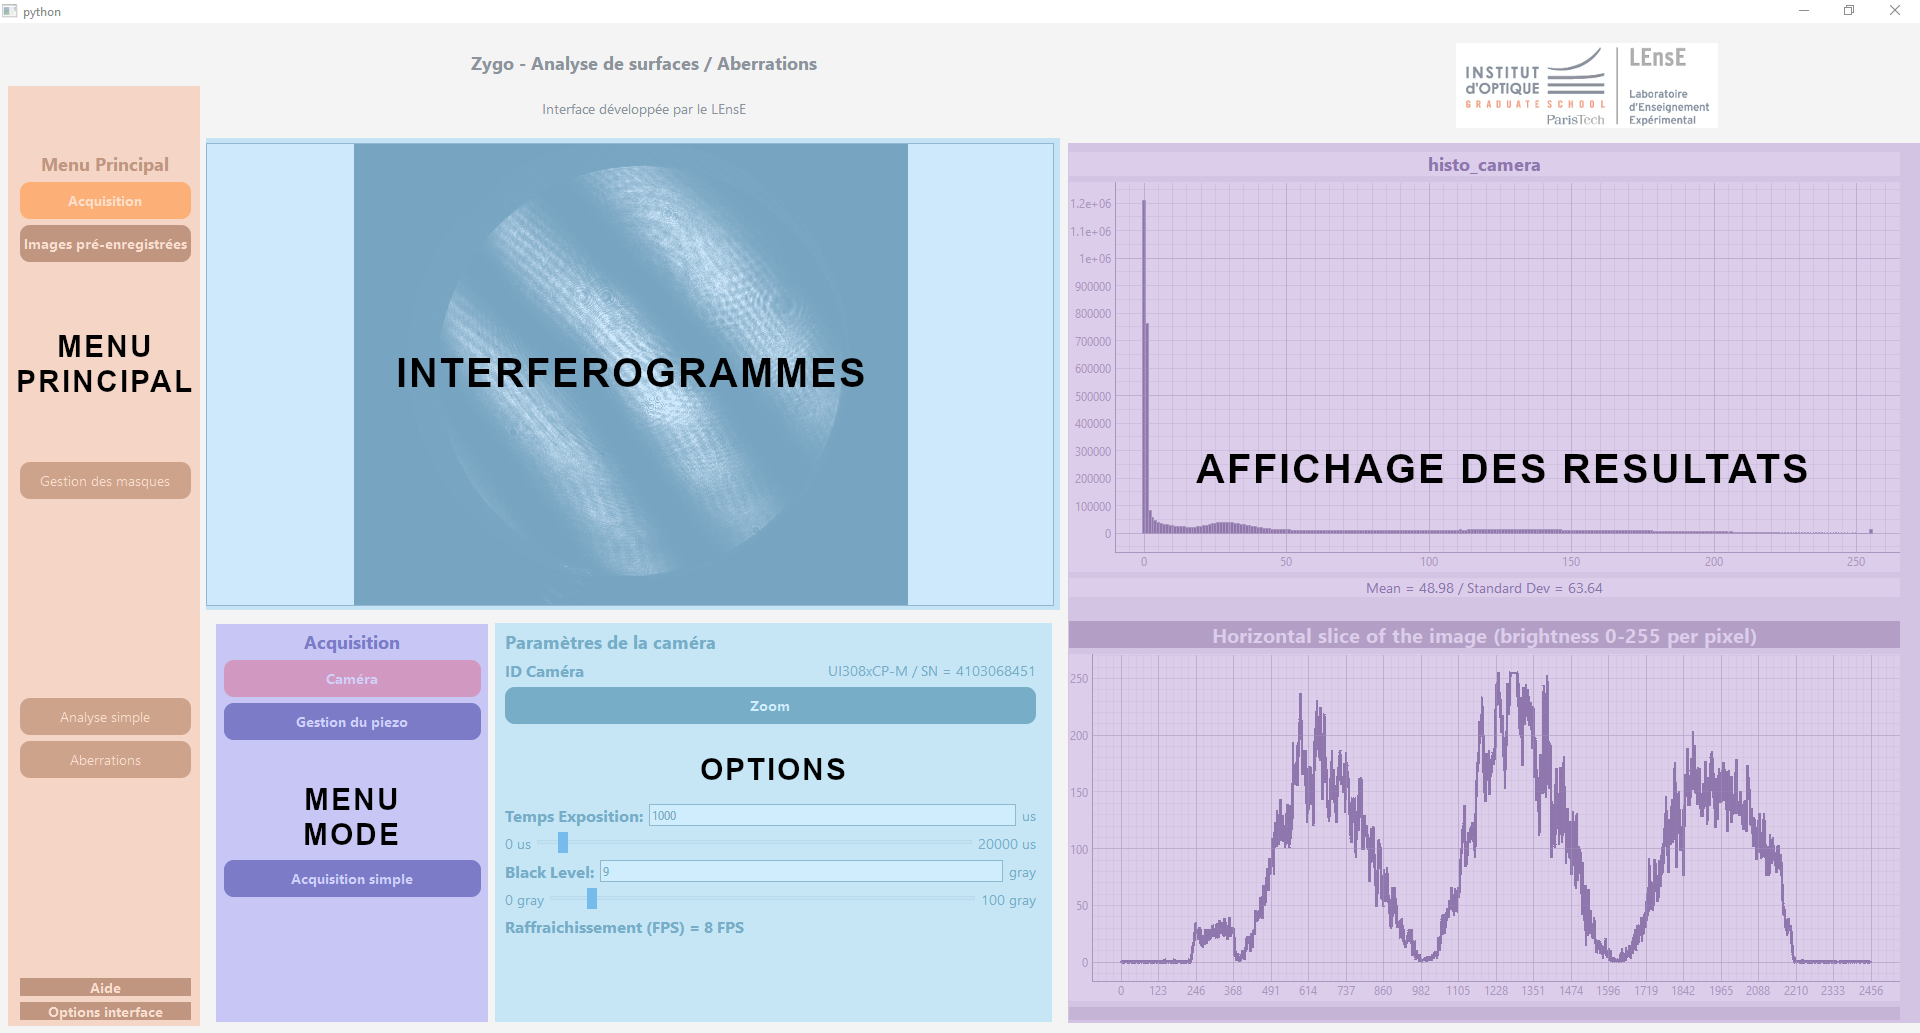
\includegraphics[width=\textwidth]{images/zygo_ihm_structure.png}
\end{center}


Il est possible d'accéder aux différentes sections de l'application par le \textbf{\textsc{menu principal}}. Chaque section de ce menu correspond à une des étapes de l'analyse.

\medskip

La partie \textbf{\textsc{Menu Mode}} affiche le menu spécifique à la section choisie dans le menu principal.

La partie \textbf{\textsc{Options}} affiche les options spécifiques à la sous-section choisie dans le menu mode.

\medskip

La partie \textbf{\textsc{Interférogrammes}} affiche (dans la plupart des étapes) l'interférogramme de référence.

La partie \textbf{\textsc{Affichage des résultats}} affiche les résultats des différents calculs proposés dans chaque section.

\medskip

Certaines options entraînent des phases de calcul un peu longues (affichage 3D, PSF...).

\bigskip


\begin{tcolorbox}[myboxstyle]
\begin{large}
\begin{center}
L'application se lance depuis le bureau par le bouton 

\begin{itemize}
	\item \textbf{\textsc{Start\_Zygo\_1A.bat}}  pour les TP sur le contrôle interférométrique
	\item \textbf{\textsc{Start\_Zygo\_2A.bat}}  pour les TP sur les aberrations
\end{itemize}

 .
\end{center}
\end{large}
\end{tcolorbox}

\bigskip

\textit{Une procédure d'installation est également proposée à la fin de ce document...}


\newpage
%%%%%%%%%%%%%%%%%%%%%%%%%%%%%%%%%%
\section{Structure de l'application}